\chapter[RESULTS AND DISCUSSION]{\huge RESULTS AND DISCUSSION}
In this chapter are shown the results from all the classification experiments performed in this work using overt and imagined speech samples. The results are shown in tables that, for simplicity,  contain the overall accuracies obtained in each case. These overall accuracies represent the sum of the training and test accuracies divided by two. In the particular cases of MLP and NeuCube, these accuracies came from the averages of the experiments with different initializations.\\

Furthermore, the experiments were conducted with the validation methodology described in the previous chapter. Due to this methodology, each row in the tables represents when a specific subject's data was held out from the rest to test the classifier (subject-independent experiments approach). Additionally, these results were obtained by the classifiers configured with the parameter's values also shown in the previous chapter.\\

Moreover, the experiments consisted of selecting the two less unbalanced data sets: $\pm$Nasal and $\pm$ Bilabial with their corresponding processing steps for the Vector-based classifiers (MLP and SVM), Spatio-Temporal classifier (NeuCube), and the Mixed approach classifier (representing it as $\mbox{SSN}_{L}$ and $\mbox{SSN}_{I}$ when LIF and Izhikevich neuron models, respectively, were used). In each section, the results from each experiment set are analyzed, and the best scores, per case, are highlighted in the tables.\\

\section{Vector-Based}
Table \ref{Table: Classification_Overt_VB} shows the overall accuracies obtained with overt speech samples using 3 or 21 features for the input vectors. For both cases, the best scores were obtained with the $\pm$Bilabial data set using the SSN with a LIF neuron model ($\mbox{SSN}_{L}$). Notice that for all the classifiers and features used, the $\pm$Bilabial data set provided better results than  $\pm$Nasal.\\

Furthermore, comparing the classifier's performances across the experiments shown in Table \ref{Table: Classification_Overt_VB}, the best were obtained with the $\mbox{SSN}_{L}$, followed by the $\mbox{SSN}_{I}$, SVM, and at last the MLP. Besides, according to these results, the use of 21 features provided slightly better results than using 3 features in the case of $\mbox{SSN}_{L}$ for rows $S_{3}$, $S_{4}$, and $S_{5}$.\\

Naturally, building vectors of 21 features implied more processing time consumption, but the SSN extracted more temporal information with 21 features than using just 3. Of course, more in-depth analysis in the future is required to select an optimal feature set to obtain both advantages: time consumption and performance.\\

\begin{table*}[h!]
	\centering
	\caption{Overall accuracies overt speech (vector-based approach).}
	\begin{tabular}{|*{10}{c|}}
		\cline{3-10}
		\multicolumn{2}{c|}{\multirow{2}{*}{}}&\multicolumn{4}{c|}{\textbf{3 FEATURES}}&\multicolumn{4}{c|}{\textbf{21 FEATURES}}\\\cline{3-10}
		\multicolumn{2}{c|}{}&\textbf{MLP}&\textbf{SVM}&\textbf{SSN}$_{L}$&\textbf{SSN}$_{I}$&\textbf{MLP}&\textbf{SVM}&\textbf{SSN}$_{L}$&\textbf{SSN}$_{I}$\\\hline
		\multirow{5}{*}{\begin{sideways}\textbf{\boldmath$\pm$\textbf{Nasal}}\end{sideways}}&\boldmath$S_{1}$&60.85 & 61.88 & 68.13 & 63.79 & 51.59 & 63.02 & 74.49 & 66.2\\\cline{2-10}
		&\boldmath$S_{2}$&59.73 & 60.72 & 67.94 & 70.32 & 52.24 & 62.64 & 70    & 67.33\\\cline{2-10}
		&\boldmath$S_{3}$&59.08 & 58.97 & 70.25 & 62.67 & 52.81 & 62.68 & 70.22 & 66.07\\\cline{2-10}
		&\boldmath$S_{4}$&59.01 & 63.71 & 71.79 & 56.37 & 53.39 & 62.86 & 68.89 & 57.68\\\cline{2-10}
		&\boldmath$S_{5}$&59.88 & 57.42 & 65.99 & 66.01 & 53.66 & 61.19 & 71.6  & 66.23\\\hline
		\multirow{5}{*}{\begin{sideways}\textbf{\boldmath$\pm$\textbf{Bilabial}}\end{sideways}}&\boldmath$S_{1}$&66.35 & 68.84 & \cellcolor{orange}75.36 & 71.25 & 52.87 & 62.84 & \cellcolor{orange}74.66 & 72.95\\\cline{2-10}
		&\boldmath$S_{2}$&67.69 & 66.14 & \cellcolor{orange}72.77 & 71.595 & 55.47 & 64.32 & \cellcolor{orange}71.99 & 71.63\\\cline{2-10}
		&\boldmath$S_{3}$&67.95 & 68.56 & \cellcolor{orange}75.42 & 74.67 & 53.6  & 62.95 & \cellcolor{orange}77.01 & 75.15\\\cline{2-10}
		&\boldmath$S_{4}$&66.67 & 67.63 & \cellcolor{orange}72.89 & 71.21 & 53.65 & 62.86 & \cellcolor{orange}73.58 & 71.21\\\cline{2-10}
		&\boldmath$S_{5}$&62.28 & 66.97 & \cellcolor{orange}70.12 & 69    & 54.21 & 59.82 & \cellcolor{orange}71.66 & 68.95\\\hline
	\end{tabular}%
	\label{Table: Classification_Overt_VB}
\end{table*}%

\begin{table*}[h!]
\centering
\caption{Overall accuracies imagined speech, 3 features (vector-based approach).}
\scalebox{0.75}{
	\begin{tabular}{|*{14}{c|}}
		\cline{3-14}
		\multicolumn{2}{c|}{\multirow{2}{*}{}}&\multicolumn{4}{c|}{\textbf{ORIGINAL}}&\multicolumn{4}{c|}{\textbf{DWT}}&\multicolumn{4}{c|}{\textbf{WPT}}\\\cline{3-14}
		\multicolumn{2}{c|}{}&\textbf{MLP}&\textbf{SVM}&\textbf{SSN}$_{L}$&\textbf{SSN}$_{I}$&\textbf{MLP}&\textbf{SVM}&\textbf{SSN}$_{L}$&\textbf{SSN}$_{I}$&\textbf{MLP}&\textbf{SVM}&\textbf{SSN}$_{L}$&\textbf{SSN}$_{I}$\\\hline
		\multirow{5}{*}{\begin{sideways}\textbf{\boldmath$\pm$\textbf{Nasal}}\end{sideways}}&\boldmath$S_{1}$&&62.91&67.65&68.13&&63.02&66.16&66.55&&63.02&65.9&66.82\\\cline{2-14}
		&\boldmath$S_{2}$&&62.6&68.19&67.16&&62.64&65.34&65.91&&62.64&65.13&67.51\\\cline{2-14}
		&\boldmath$S_{3}$&&62.63&74.2&65.36&&62.68&68.5&66.76&&62.68&68.02&67.39\\\cline{2-14}
		&\boldmath$S_{4}$&&62.82&66.27&64.62&&62.86&68.76&65.35&&62.86&64.51&65.46\\\cline{2-14}
		&\boldmath$S_{5}$&&61.16&64.7&62.94&&61.19&68.04&68.29&&61.19&63.77&67.03\\\hline
		\multirow{5}{*}{\begin{sideways}\textbf{\boldmath$\pm$\textbf{Bilabial}}\end{sideways}}&\boldmath$S_{1}$&58.62&64.32&\cellcolor{orange}69.72&69.67&51.81&62.85&65.06&68.39&51.62&62.85&65.06&68.17\\\cline{2-14}
		&\boldmath$S_{2}$&57.98&64.92&\cellcolor{orange}69.86&72.34&56.21&64.32&69&72.12&54.39&62.12&66.96&70.53\\\cline{2-14}
		&\boldmath$S_{3}$&59.71&62.9&\cellcolor{orange}75.67&74.03&55.7&62.95&65.41&66.37&54.39&62.95&65.65&66.61\\\cline{2-14}
		&\boldmath$S_{4}$&58.37&63.81&\cellcolor{orange}77.79&69.72&59.37&62.86&68.11&68.12&58.95&62.86&65.97&68.58\\\cline{2-14}
		&\boldmath$S_{5}$&56.97&59.78&\cellcolor{orange}66.9&67.69&57.52&59.82&66.01&65.82&55.75&59.82&62.51&66.51\\\hline
	\end{tabular}%
}
\label{Table: Classification_Imagined_3feats_VB}
\end{table*}%

On the other hand, Tables \ref{Table: Classification_Imagined_3feats_VB} and \ref{Table: Classification_Imagined_21feats_VB} show the overall accuracies obtained with imagined speech samples using 3 and 21 features, respectively, for the input vectors.\\

Due to the processing step with wavelets, imagined speech results were split into two tables, in which the "Original" column referred to when features were extracted from the EEG signal without wavelet processing. While the other columns represent the scores obtained with vectors composed of PCA components from DWT or WPT feature vectors.\\

Besides, similar to overt speech experiments, the best accuracies obtained were with $\pm$Bilabial data sets and $\mbox{SSN}_{L}$ classifier. However, these best results, based on the data set used, varied for the other classifiers, particularly for the $\mbox{SSN}_{I}$ in which$\pm$Nasal data set provided better accuracies in some cases.\\

Also, the best scores obtained with 3 and 21 features came from original signals (no wavelets usage). These results might mean that the mother wavelet was not adequated for these data and further experiments with other wavelet mothers are required.\\

\begin{table*}[h!]
\centering
\caption{Overall accuracies imagined speech, 21 features (vector-based approach).}
\scalebox{0.75}{
	\begin{tabular}{|*{14}{c|}}
		\cline{3-14}
		\multicolumn{2}{c|}{\multirow{2}{*}{}}&\multicolumn{4}{c|}{\textbf{ORIGINAL}}&\multicolumn{4}{c|}{\textbf{DWT}}&\multicolumn{4}{c|}{\textbf{WPT}}\\\cline{3-14}
		\multicolumn{2}{c|}{}&\textbf{MLP}&\textbf{SVM}&\textbf{SSN}$_{L}$&\textbf{SSN}$_{I}$&\textbf{MLP}&\textbf{SVM}&\textbf{SSN}$_{L}$&\textbf{SSN}$_{I}$&\textbf{MLP}&\textbf{SVM}&\textbf{SSN}$_{L}$&\textbf{SSN}$_{I}$\\\hline
		\multirow{5}{*}{\begin{sideways}\textbf{\boldmath$\pm$\textbf{Nasal}}\end{sideways}}&\boldmath$S_{1}$&&62.91&66.73&65.33&&63.02&69.36&67.52&&63.02&69.49&68.39\\\cline{2-14}
		&\boldmath$S_{2}$&&62.6&64.13&64.81&&62.64&65.13&67.26&&62.64&65.02&67.55\\\cline{2-14}
		&\boldmath$S_{3}$&&62.63&64.31&65.99&&62.68&67.88&70.43&&62.68&72.69&67.42\\\cline{2-14}
		&\boldmath$S_{4}$&&62.82&61.34&64.48&&62.86&72.65&66.69&&62.86&66.11&66.81\\\cline{2-14}
		&\boldmath$S_{5}$&&61.16&63.38&63.16&&61.19&65.03&64.78&&61.19&65.66&64.53\\\hline
		\multirow{5}{*}{\begin{sideways}\textbf{\boldmath$\pm$\textbf{Bilabial}}\end{sideways}}&\boldmath$S_{1}$&&62.73&\cellcolor{orange}68.14&71.61&&62.85&68.83&68.92&&62.85&69.4&70.14\\\cline{2-14}
		&\boldmath$S_{2}$&&64.28&\cellcolor{orange}68.37&70.79&&64.32&68.89&69.15&&64.32&71.42&72.17\\\cline{2-14}
		&\boldmath$S_{3}$&&62.9&\cellcolor{orange}77.02&74.56&&62.95&67.9&66.91&&62.95&68.69&67.9\\\cline{2-14}
		&\boldmath$S_{4}$&&62.82&\cellcolor{orange}75.02&72.49&&62.86&70.77&67.49&&62.86&71.46&66.11\\\cline{2-14}
		&\boldmath$S_{5}$&&59.78&\cellcolor{orange}67.3&66.18&&59.82&63.36&65.91&&59.82&63.69&67.71\\\hline
	\end{tabular}%
}
\label{Table: Classification_Imagined_21feats_VB}
\end{table*}%

Furthermore, comparing the performances obtained across the experiments, the classifier that provided the best accuracies was the SSN (the neuron model varied per case), followed by the SVM and at last the MLP. While comparing the feature's set used, similar to overt speech samples, the results using 3 and 21 features were similar. However, these results were worse than those obtained with overt speech samples in this approach (Vector-based).\\

\section{Spatio-Temporal}
In this section are analyzed the results obtained with the Spatio-temporal classifiers used in this work: NeuCube and SSN (with LIF and Izhikevich neuron models). Table \ref{Table: Classification_ST} summarizes these results for overt and imagined speech samples. Notice that, as in the Vector-based approach, the best results (highlighted) were provided by a $\pm$Bilabial data set using the $\mbox{SSN}_{L}$ classifier.\\

Besides, the best scores provided by each classifier were obtained from the $\pm$Bilabial data set, except for the NeuCube by using overt speech samples in which $\pm$Nasal data set provided slightly better results than $\pm$Bilabial. Furthermore, in some cases, the $\mbox{SSN}_{I}$  provided better results than the $\mbox{SSN}_{L}$. For this reason, the results from both classifier models are detailed and compared in the next section. In this section, just NeuCube results are analyzed.\\

Although grid searches were performed for the NeuCube, their accuracies, compared with the SSNs results, were the worst in these experiments. These low performances occurred due to the few grid searches performed, and the few parameters explored. In the previous chapter was explained that two grid searches (corresponding to $\pm$Nasal and $\pm$Bilabial data sets) per mental activity (overt and imagined) were performed twice each.\\

By contrast, the optimization process in the SSN was performed for all the case\linebreak[4] individually (corresponding to each cell in Table \ref{Table: Classification_ST})). However, a grid search or an optimization process (similar to that with the SSN) per case was not possible with the NeuCube due to time consumption. The NeuCube has several parameters and processes that would have implied many computations out of scope for time limitations in this work if an optimization process had been performed.\\

\begin{table}[h!]
	\centering
	\caption{Overall accuracies overt and imagined speech (spatio-temporal approach).}
	\begin{tabular}{|*{8}{c|}}
		\cline{3-8}
		\multicolumn{2}{c|}{\multirow{2}{*}{}}&\multicolumn{3}{c|}{\textbf{OVERT SPEECH}}&\multicolumn{3}{c|}{\textbf{IMAGINED SPEECH}}\\\cline{3-8}
		\multicolumn{2}{c|}{}&\textbf{NeuCube}&\textbf{SSN}$_{L}$&\textbf{SSN}$_{I}$&\textbf{NeuCube}&\textbf{SSN}$_{L}$&\textbf{SSN}$_{I}$\\\hline
		\multirow{5}{*}{\begin{sideways}\textbf{$\pm$\textbf{Nasal}}\end{sideways}}&\boldmath$S_{1}$&58.69 & 71.06 & 66.02 & 55.97 & 64.27 & 65.85 \\\cline{2-8}
		&\boldmath$S_{2}$&58.89 & 64.16 & 62.18 & 57.83 & 64.35 & 64.74\\\cline{2-8}
		&\boldmath$S_{3}$&57.09 & 66.53 & 67.06 & 56.93 & 67.41 & 64.59\\\cline{2-8}
		&\boldmath$S_{4}$&60.32 & 71.79 & 66.87 & 58.07 & 65.93 & 62.68\\\cline{2-8}
		&\boldmath$S_{5}$&61.21 & 69.47 & 65.38 & 55.32 & 62.67 & 62.78\\\hline
		\multirow{5}{*}{\begin{sideways}\textbf{\boldmath$\pm$\textbf{Bilabial}}\end{sideways}}&\boldmath$S_{1}$&58.69 & \cellcolor{orange}68.65 & 72.43 & 58.49 & \cellcolor{orange}72.03 & 69.93\\\cline{2-8}
		&\boldmath$S_{2}$&58.12 & \cellcolor{orange}71.14 & 74.13 & 57.22 & \cellcolor{orange}72.66 & 71.78\\\cline{2-8}
		&\boldmath$S_{3}$&56.63 & \cellcolor{orange}74.73 & 71.76 & 58.15 & \cellcolor{orange}77.57 & 73.85\\\cline{2-8}
		&\boldmath$S_{4}$&58.99 & \cellcolor{orange}70.92 & 69.47 & 58.64 & \cellcolor{orange}75.09 & 68.08\\\cline{2-8}
		&\boldmath$S_{5}$&55.01 & \cellcolor{orange}73.21 & 66.18 & 54.63 & \cellcolor{orange}70.43 & 65.49\\\hline
		\end{tabular}%
		\label{Table: Classification_ST}
\end{table}%

\begin{table}[h!]
	\centering
	\caption{NeuCube accuracies for overt speech samples using $\pm$Nasal data set.}
	\scalebox{0.53}{
	\begin{tabular}{|*{11}{c|}}
		\hline
		\textbf{Subject} & \multicolumn{2}{c|}{\boldmath$S_{1}$} & \multicolumn{2}{c|}{\boldmath$S_{2}$} & \multicolumn{2}{c|}{\boldmath$S_{3}$} & \multicolumn{2}{c|}{\boldmath$S_{4}$} & \multicolumn{2}{c|}{\boldmath$S_{5}$} \\\hline
		\textbf{Init.} & \textbf{Training} & \textbf{Test} &  \textbf{Training} & \textbf{Test} & \textbf{Training} & \textbf{Test} & \textbf{Training} & \textbf{Test} & \textbf{Training} & \textbf{Test} \\\hline
		1 & 57.11 & 65.03 & 60.77 & 52.70 & 61.93 & 59.38 & 56.89 & 62.79 & 58.99 & 60.92 \\\hline
		2 & 60.26 & 54.60 & 60.13 & 62.16 & 59.28 & 47.66 & 60.18 & 65.12 & 60.53 & 58.62 \\\hline
		3 & 58.16 & 52.76 & 62.05 & 48.65 & 60.96 & 42.97 & 59.96 & 54.65 & 60.75 & 62.07 \\\hline
		4 & 60.26 & 60.12 & 61.41 & 58.11 & 61.45 & 54.69 & 58.86 & 59.30 & 58.33 & 59.77 \\\hline
		5 & 61.58 & 56.44 & 58.42 & 54.05 & 60.24 & 56.25 & 59.74 & 55.81 & 58.77 & 57.47 \\\hline
		6 & 56.05 & 48.47 & 61.19 & 59.46 & 62.89 & 47.66 & 61.71 & 59.30 & 60.31 & 54.02 \\\hline
		7 & 63.42 & 61.35 & 58.21 & 58.11 & 65.78 & 41.41 & 61.49 & 55.81 & 64.25 & 62.07 \\\hline
		8 & 61.84 & 53.99 & 59.28 & 56.76 & 65.54 & 42.19 & 58.64 & 56.98 & 61.62 & 68.97 \\\hline
		9 & 59.21 & 49.69 & 62.05 & 59.46 & 58.07 & 50.78 & 64.99 & 58.14 & 62.72 & 62.07 \\\hline
		10 & 62.37 & 60.12 & 62.26 & 50.00 & 64.58 & 52.34 & 56.89 & 63.95 & 58.99 & 64.37 \\\hline
		11 & 57.63 & 58.90 & 62.47 & 54.05 & 60.72 & 53.13 & 63.24 & 54.65 & 64.25 & 59.77 \\\hline
		12 & 58.68 & 61.96 & 62.47 & 58.11 & 61.45 & 58.59 & 61.27 & 65.12 & 61.62 & 64.37 \\\hline
		13 & 54.47 & 52.76 & 60.98 & 62.16 & 63.86 & 52.34 & 62.36 & 55.81 & 59.43 & 57.47 \\\hline
		14 & 60.00 & 65.64 & 60.98 & 68.92 & 61.93 & 56.25 & 59.30 & 58.14 & 60.31 & 64.37 \\\hline
		15 & 61.32 & 63.19 & 59.49 & 62.16 & 64.58 & 59.38 & \cellcolor{orange}62.36 & \cellcolor{orange}65.12 & 59.21 & 60.92 \\\hline
		16 & 57.37 & 58.28 & 59.70 & 63.51 & 58.80 & 49.22 & 61.49 & 65.12 & 58.33 & 60.92 \\\hline
		17 & 60.53 & 56.44 & 62.26 & 62.16 & 63.86 & 54.69 & 61.71 & 55.81 & 61.18 & 64.37 \\\hline
		18 & 60.26 & 61.35 & 57.78 & 58.11 & 61.69 & 58.59 & 62.58 & 56.98 & 62.28 & 63.22 \\\hline
		19 & 58.16 & 53.37 & 57.14 & 48.65 & 60.48 & 51.56 & 59.96 & 65.12 & 64.04 & 57.47 \\\hline
		20 & 60.53 & 63.80 & 56.50 & 52.70 & 61.20 & 55.47 & 60.18 & 65.12 & 59.21 & 70.11 \\\hline
		\textbf{Avg.} & \textbf{59.46}\boldmath$\pm$\textbf{2.25} & \textbf{57.91}\boldmath$\pm$\textbf{5.05} & \textbf{60.28}\boldmath$\pm$\textbf{1.88} & \textbf{57.5}\boldmath$\pm$\textbf{5.36} & \textbf{61.96}\boldmath$\pm$\textbf{2.18} & \textbf{52.23}\boldmath$\pm$\textbf{5.6} & \textbf{60.69}\boldmath$\pm$\textbf{2.03} & \textbf{59.94}\boldmath$\pm$\textbf{4.19} & \textbf{60.76}\boldmath$\pm$\textbf{1.95} & \textbf{61.67}\boldmath$\pm$\textbf{3.88} \\\hline
	\end{tabular}%
	}
	\label{Table: NeuCube_Overt_Accuracies}%
\end{table}%

Also, Table \ref{Table: NeuCube_Overt_Accuracies} shows each classification accuracy, as well as their averages $\pm$ the standard deviation, obtained with 20 different initializations for the NeuCube using overt speech samples and configured with the $\pm$Nasal data set (the best results obtained for this case, according to the overall accuracies shown in Table \ref{Table: Classification_ST}).\\

On the other hand, Tables \ref{Table: NeuCube_Imagined_Accuracies1} and \ref{Table: NeuCube_Imagined_Accuracies2}  show the same information as in Table \ref{Table: NeuCube_Overt_Accuracies} but from the experiments that used $\pm$Bilabial configured imagined speech samples with the highlighted parameters for overt and imagined speech samples in Table \ref{Table: NeuCube_Gridsearch_Values}, respectively.\\

Hence, the overall accuracies shown in Table \ref{Table: Classification_ST} came from the Table \ref{Table: NeuCube_Imagined_Accuracies1} values because they were higher than those from Table \ref{Table: NeuCube_Imagined_Accuracies2}. Furthermore, the most balanced cases of training and test accuracies with the NeuCube were selected from Tables \ref{Table: NeuCube_Overt_Accuracies} and \ref{Table: NeuCube_Imagined_Accuracies1} (those highlighted) to show their firing activities and weight's distributions.\\

\begin{table}[h!]
	\centering
	\caption{NeuCube accuracies for imagined speech samples using $\pm$Bilabial data set (1st parameter set).}
	\scalebox{0.53}{
		\begin{tabular}{|*{11}{c|}}
			\hline
			\textbf{Subject} & \multicolumn{2}{c|}{\boldmath$S_{1}$} & \multicolumn{2}{c|}{\boldmath$S_{2}$} & \multicolumn{2}{c|}{\boldmath$S_{3}$} & \multicolumn{2}{c|}{\boldmath$S_{4}$} & \multicolumn{2}{c|}{\boldmath$S_{5}$} \\\hline
			\textbf{Init.} & \textbf{Training} & \textbf{Test} &  \textbf{Training} & \textbf{Test} & \textbf{Training} & \textbf{Test} & \textbf{Training} & \textbf{Test} & \textbf{Training} & \textbf{Test} \\\hline
			1 & 61.05 & 52.76 & 65.46 & 55.41 & 56.14 & 57.81 & 63.68 & 58.14 & 63.16 & 42.53 \\\hline
			2 & 60.79 & 57.67 & 60.13 & 56.76 & 60.72 & 60.94 & 61.49 & 45.35 & 59.65 & 47.13 \\\hline
			3 & 59.21 & 51.53 & 61.19 & 56.76 & 58.55 & 64.06 & 58.42 & 59.30 & 65.35 & 47.13 \\\hline
			4 & 57.11 & 49.08 & 61.19 & 43.24 & 61.20 & 53.91 & 59.08 & 60.47 & 64.04 & 47.13 \\\hline
			5 &61.32 & 38.65 & 62.05 & 51.35 & 56.14 & 65.63 & 61.27 & 51.16 & 64.47 & 49.43 \\\hline
			6 & 62.11 & 58.28 & 62.69 & 59.46 & 57.11 & 58.59 & 62.58 & 52.33 & 62.94 & 48.28 \\\hline
			7 & 64.47 & 60.74 & 60.98 & 55.41 & 53.98 & 64.84 & 59.96 & 55.81 & 66.45 & 50.57 \\\hline
			8 & 60.79 & 53.37 & 60.34 & 64.86 & 57.11 & 55.47 & 58.42 & 63.95 & 60.75 & 50.57 \\\hline
			9 & 59.47 & 64.42 & 60.55 & 55.41 & 59.04 & 58.59 & 63.24 & 53.49 & 62.06 & 41.38 \\\hline
			10 & 64.47 & 65.64 & 61.83 & 40.54 & 60.00 & 57.81 & 59.30 & 59.30 & 62.28 & 44.83 \\\hline
			11 & 60.79 & 66.26 & 63.33 & 48.65 & 61.45 & 59.38 & 58.42 & 56.98 & 61.40 & 50.57 \\\hline
			12 & 63.68 & 60.12 & 66.10 & 56.76 & 58.31 & 63.28 & 60.61 & 58.14 & 63.16 & 49.43 \\\hline
			13 & 64.47 & 53.99 & 57.57 & 43.24 & 56.87 & 58.59 & 61.93 & 55.81 & 62.50 & 48.28 \\\hline
			14 & 64.21 & 46.63 & 63.75 & 59.46 & 56.14 & 53.91 & 63.68 & 50.00 & 60.09 & 43.68 \\\hline
			15 & 60.53 & 46.63 & 62.26 & 37.84 & 58.07 & 61.72 & 62.80 & 52.33 & 62.72 & 52.87 \\\hline
			16 & \cellcolor{orange}65.26 & \cellcolor{orange}62.58 & 62.05 & 55.41 & 59.52 & 55.47 & 58.64 & 58.14 & 60.75 & 48.28 \\\hline
			17 & 62.11 & 52.76 & 61.62 & 58.11 & 62.17 & 46.09 & 62.14 & 54.65 & 62.06 & 49.43 \\\hline
			18 & 61.32 & 49.69 & 62.90 & 67.57 & 58.07 & 61.72 & 61.49 & 60.47 & 62.06 & 37.93 \\\hline
			19 & 64.21 & 55.83 & 60.98 & 50.00 & 56.14 & 51.56 & 61.49 & 60.47 & 63.38 & 36.78 \\\hline
			20 & 58.16 & 57.67 & 60.55 & 35.14 & 56.63 & 53.13 & 57.77 & 62.79 & 63.82 & 45.98 \\\hline
			\textbf{Avg.} & \textbf{61.78}\boldmath$\pm$\textbf{2.32} & \textbf{55.21}\boldmath$\pm$\textbf{7.13} & \textbf{61.88}\boldmath$\pm$\textbf{1.89} & \textbf{52.57}\boldmath$\pm$\textbf{8.73} & \textbf{58.17}\boldmath$\pm$\textbf{2.16} & \textbf{58.12}\boldmath$\pm$\textbf{4.93} & \textbf{60.82}\boldmath$\pm$\textbf{1.93} & \textbf{56.45}\boldmath$\pm$\textbf{4.64} & \textbf{62.65}\boldmath$\pm$\textbf{1.7} & \textbf{46.61}\boldmath$\pm$\textbf{4.28} \\\hline
		\end{tabular}%
	}
	\label{Table: NeuCube_Imagined_Accuracies1}%
\end{table}%

\begin{table}[h!]
	\centering
	\caption{NeuCube accuracies for imagined speech samples using $\pm$Bilabial data set (2nd parameter set).}
	\scalebox{0.53}{
		\begin{tabular}{|*{11}{c|}}
			\hline
			\textbf{Subject} & \multicolumn{2}{c|}{\boldmath$S_{1}$} & \multicolumn{2}{c|}{\boldmath$S_{2}$} & \multicolumn{2}{c|}{\boldmath$S_{3}$} & \multicolumn{2}{c|}{\boldmath$S_{4}$} & \multicolumn{2}{c|}{\boldmath$S_{5}$} \\\hline
			\textbf{Init.} & \textbf{Training} & \textbf{Test} &  \textbf{Training} & \textbf{Test} & \textbf{Training} & \textbf{Test} & \textbf{Training} & \textbf{Test} & \textbf{Training} & \textbf{Test} \\\hline
			1 & 62.11 & 52.15 & 62.26 & 55.41 & 55.66 & 60.16 & 62.58 & 61.63 & 61.62 & 42.53 \\\hline
			2 & 65.79 & 50.92 & 58.00 & 60.81 & 53.49 & 49.22 & 57.33 & 52.33 & 64.04 & 42.53 \\\hline
			3 & 62.63 & 52.15 & 60.13 & 54.05 & 60.72 & 60.94 & 63.68 & 51.16 & 59.87 & 44.83 \\\hline
			4 & 62.89 & 56.44 & 61.83 & 59.46 & 58.31 & 54.69 & 59.08 & 58.14 & 62.28 & 45.98 \\\hline
			5 & 63.68 & 52.76 & 61.83 & 52.70 & 59.04 & 59.38 & 62.36 & 58.14 & 59.21 & 43.68 \\\hline
			6 & 63.42 & 54.60 & 62.47 & 44.59 & 57.11 & 58.59 & 61.27 & 61.63 & 59.87 & 44.83 \\\hline
			7 & 61.05 & 60.12 & 62.69 & 51.35 & 57.59 & 56.25 & 59.74 & 51.16 & 67.32 & 42.53 \\\hline
			8 & 60.53 & 33.74 & 60.13 & 51.35 & 60.48 & 56.25 & 60.39 & 52.33 & 64.69 & 47.13 \\\hline
			9 & 70.00 & 39.26 & 58.64 & 55.41 & 60.00 & 56.25 & 61.27 & 60.47 & 62.06 & 50.57 \\\hline
			10 & 60.26 & 61.35 & 56.08 & 45.95 & 60.24 & 60.94 & 62.58 & 53.49 & 62.72 & 39.08 \\\hline
			11 & 60.79 & 37.42 & 61.83 & 52.70 & 56.63 & 54.69 & 63.02 & 54.65 & 65.13 & 48.28 \\\hline
			12 & 62.37 & 55.21 & 60.55 & 36.49 & 57.11 & 64.06 & 63.68 & 43.02 & 58.55 & 36.78 \\\hline
			13 & 62.63 & 64.42 & 64.39 & 52.70 & 56.39 & 58.59 & 63.89 & 56.98 & 63.38 & 35.63 \\\hline
			14 & 61.32 & 44.17 & 62.05 & 44.59 & 59.52 & 60.16 & 58.86 & 48.84 & 62.06 & 43.68 \\\hline
			15 & 59.74 & 57.67 & 60.77 & 52.70 & 58.55 & 59.38 & 62.58 & 58.14 & 59.43 & 50.57 \\\hline
			16 & 56.84 & 44.79 & 61.41 & 64.86 & 59.28 & 54.69 & 60.39 & 61.63 & 59.21 & 42.53 \\\hline
			17 & 63.95 & 63.80 & 65.88 & 43.24 & 60.00 & 57.81 & 61.71 & 58.14 & 62.06 & 42.53 \\\hline
			18 & 60.79 & 35.58 & 58.85 & 52.70 & 57.11 & 57.81 & 60.61 & 59.30 & 63.16 & 43.68 \\\hline
			19 & 62.11 & 53.37 & 55.86 & 54.05 & 59.76 & 58.59 & 59.30 & 53.49 & 65.35 & 45.98 \\\hline
			20 & 63.68 & 58.28 & 60.55 & 47.30 & 53.25 & 63.28 & 60.39 & 55.81 & 59.65 & 55.17 \\\hline
			\textbf{Avg.} & \textbf{62.3}\boldmath$\pm$\textbf{2.62} & \textbf{51.41}\boldmath$\pm$\textbf{9.29} & \textbf{60.81}\boldmath$\pm$\textbf{2.48} & \textbf{51.62}\boldmath$\pm$\textbf{6.56} & \textbf{58.01}\boldmath$\pm$\textbf{2.18} & \textbf{58.09}\boldmath$\pm$\textbf{3.37} & \textbf{61.24}\boldmath$\pm$\textbf{1.82} & \textbf{55.52}\boldmath$\pm$\textbf{4.86} & \textbf{62.08}\boldmath$\pm$\textbf{2.44} & \textbf{44.43}\boldmath$\pm$\textbf{4.6} \\\hline
		\end{tabular}%
	}
	\label{Table: NeuCube_Imagined_Accuracies2}%
\end{table}%

Figures \ref{Fig: NeuCube_FA_Overt} and \ref{Fig: NeuCube_FA_Imagined} show, the initial and final (post-training) firing activities from each NeuCube connection by feeding them with overt and imagined speech samples, respectively.\\

In both cases, the firing activities at the top of the plots correspond to the connections between input neurons and other reservoir neurons, while those from the bottom represents the output connections. For this reason, such firing activities were the most saturated, even with the initial weights (top plots from Figures \ref{Fig: NeuCube_FA_Overt} and \ref{Fig: NeuCube_FA_Imagined}).\\

Besides, in both figures seems that those connections with initial high firing activity became more saturated after training the NeuCube. On the other hand, those connections with few or no activity in the initial step remained with no firing activity after the training step, which means that the information did not propagate through those connections.\\

\begin{figure}[h!]
\centering
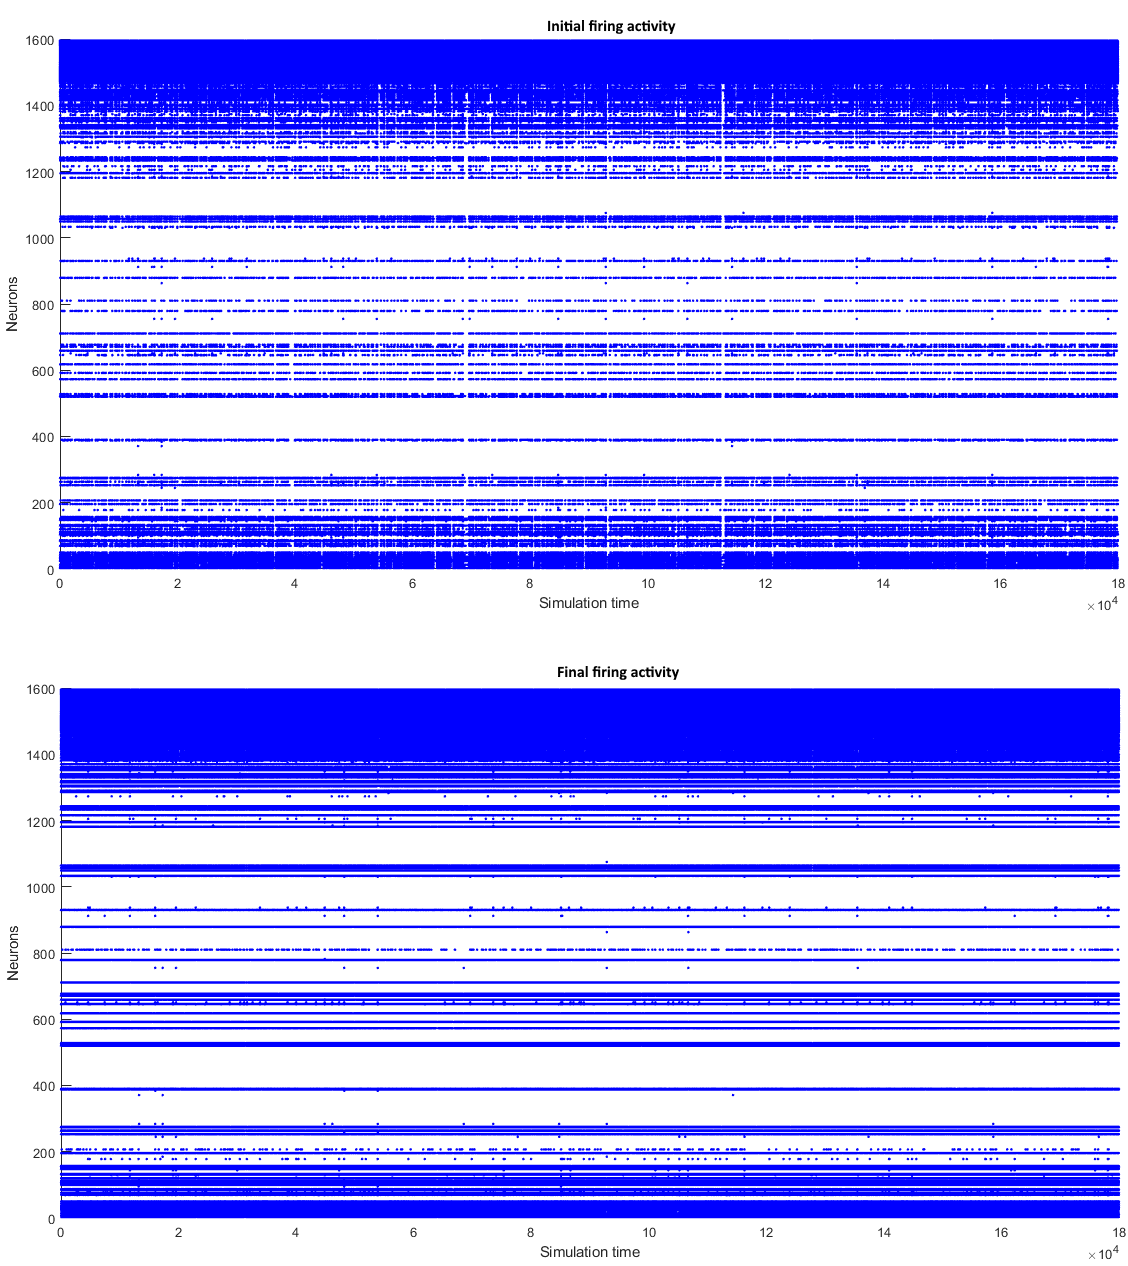
\includegraphics[width=\linewidth]{Figures/NeuCube_FA_Overt.png}
\caption{Initial and final firing activity with the NeuCube using overt speech samples.}
\label{Fig: NeuCube_FA_Overt}
\end{figure}

Moreover, Figures \ref{Fig: NeuCube_Weights_Overt} and \ref{Fig: NeuCube_Weights_Imagined} show, respectively, for overt and imagined speech samples the initial and final weight's distributions from the same highlighted cases in Tables \ref{Table: NeuCube_Overt_Accuracies} and \ref{Table: NeuCube_Imagined_Accuracies1}.  Thus, at the top of the distributions are shown the amount of positive ($p$), negative ($n$), and zero ($z$) weight's values.\\

Notice that the initial distributions in both Figures were similar due to the value selected for $r_{+}$, which set 30\% of the connections as excitatory (positives) and 70\% as inhibitory (negatives). Hence, in both Figures, the final distribution shows that most of the weight's values are close to zero, except for some weights that presented values of -2.\\

\begin{figure}[h!]
\centering
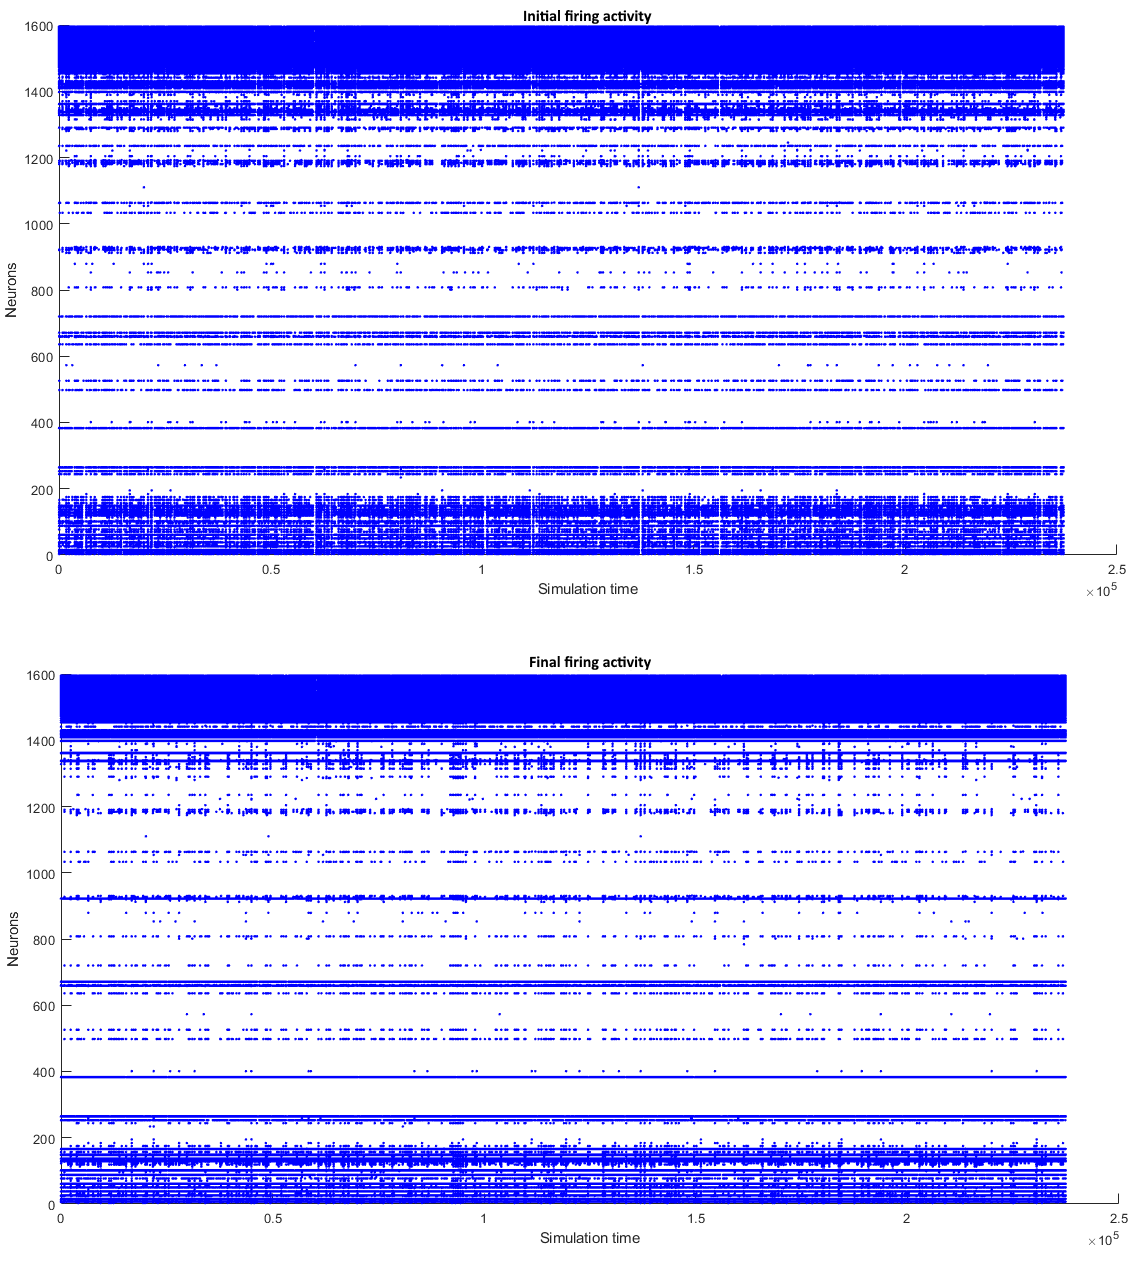
\includegraphics[width=\linewidth]{Figures/NeuCube_FA_Imagined.png}
\caption{Initial and final firing activity with the NeuCube using imagined speech samples.}
\label{Fig: NeuCube_FA_Imagined}
\end{figure}

\begin{figure}[h!]
\centering
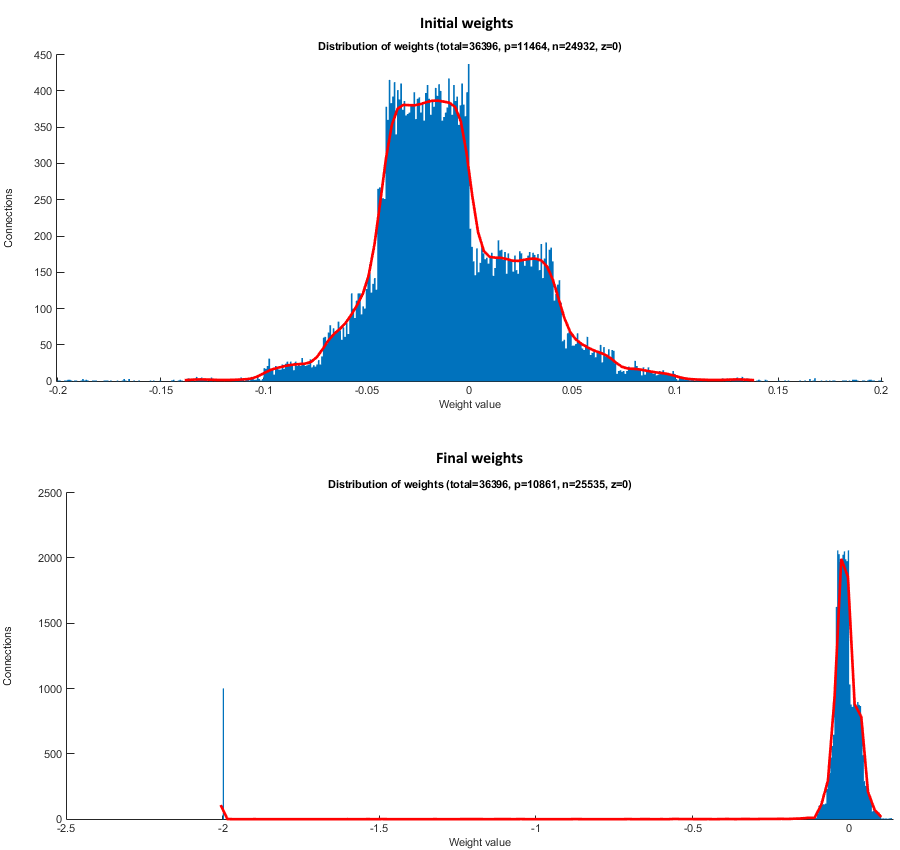
\includegraphics[scale=0.44]{Figures/NeuCube_Weights_Overt.png}
\caption{Initial and final weights with the NeuCube using overt speech samples.}
\label{Fig: NeuCube_Weights_Overt}
\end{figure}

\begin{figure}[h!]
\centering
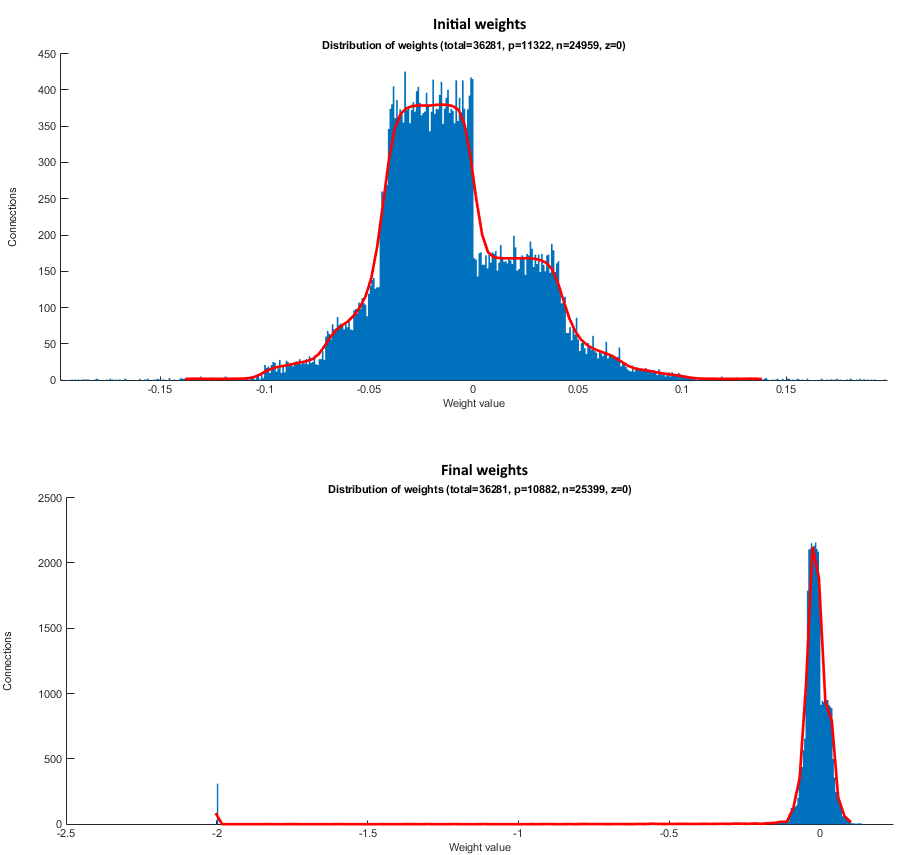
\includegraphics[scale=0.44]{Figures/NeuCube_Weights_Imagined.png}
\caption{Initial and final weights with the NeuCube using imagined speech samples.}
\label{Fig: NeuCube_Weights_Imagined}
\end{figure}

\begin{figure}[h!]
\centering
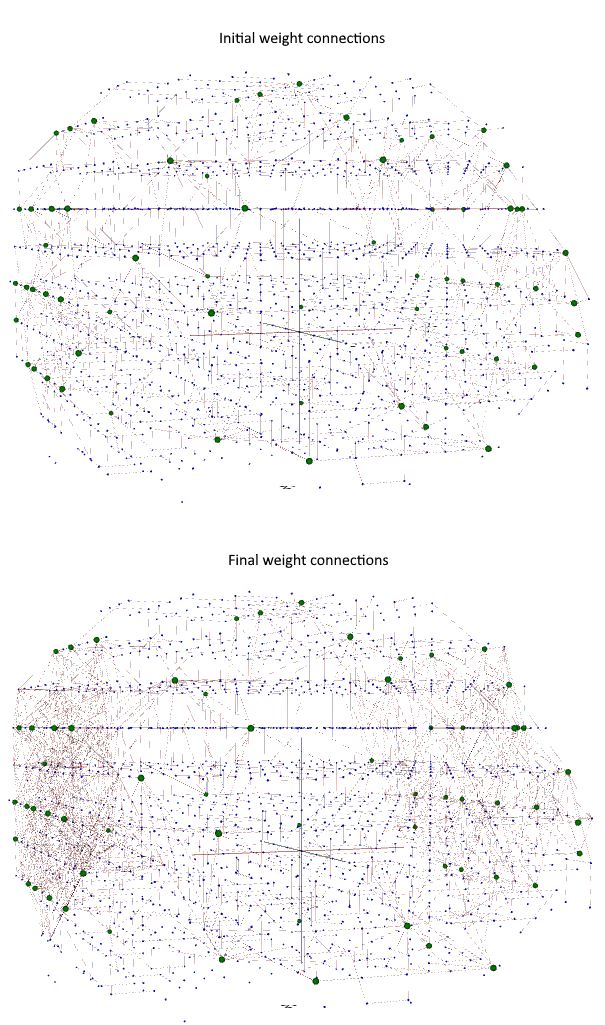
\includegraphics[scale=0.77]{Figures/NeuCube_Connections_Overt.png}
\caption{Initial and final NeuCube connections for overt speech samples.}
\label{Fig: NeuCube_Connections_Overt}
\end{figure}

\begin{figure}[h!]
\centering
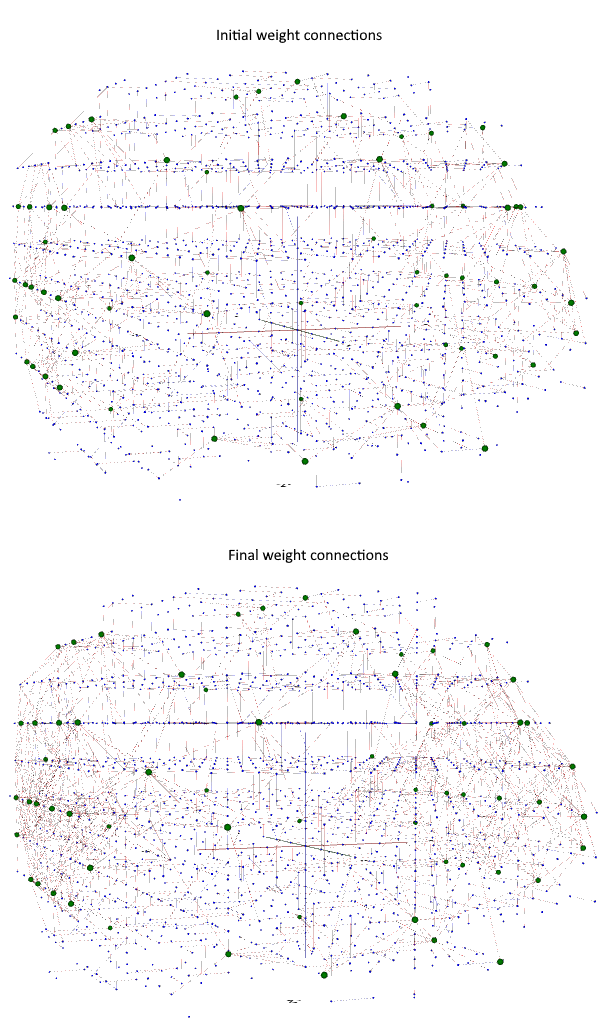
\includegraphics[scale=0.77]{Figures/NeuCube_Connections_Imagined.png}
\caption{Initial and final NeuCube connections for imagined speech samples.}
\label{Fig: NeuCube_Connections_Imagined}
\end{figure}

Furthermore, in Figures \ref{Fig: NeuCube_Connections_Overt} and \ref{Fig: NeuCube_Connections_Imagined} are shown the initial (pre-training) and final\linebreak[4] (post-training) weight's connections for the cases exposed here of overt and imagined speech samples, respectively.\\

In both Figures, the green points represent the input neurons, while the blue points are the reservoir neurons. Indeed, all neuron's locations are based on the Talareich template, which has a total of 1471 neurons.\\

Hence, the blue and red lines represent the excitatory and inhibitory connections, respectively. Notice that there are more inhibitory than excitatory connections in both Figures, particularly on the initial reservoir, which match with the weight's distributions shown in Figures \ref{Fig: NeuCube_Weights_Overt} and \ref{Fig: NeuCube_Weights_Imagined}.\\

Also, in both Figures, more connections are represented in the final reservoir plots than in the initial. These behaviors happened because just the connections with weights below -0.7 and above 0.7 are shown, and, according to Figures \ref{Fig: NeuCube_Weights_Overt} and \ref{Fig: NeuCube_Weights_Imagined}, the initial weight's distribution was sparer than the final, which caused more weights discrimination when the interval was selected.\\

To sum up, the firing activities from Figures \ref{Fig: NeuCube_FA_Overt} and \ref{Fig: NeuCube_FA_Imagined} shown that the information did not pass through the reservoir, just in the input connections and some few others. This argument is reinforced with the final connections shown in Figures \ref{Fig: NeuCube_Connections_Overt} and \ref{Fig: NeuCube_Connections_Imagined}. Due to that, the NeuCube has failed in many recognitions for training and test data. Besides, the grid search was performed with few cases, with which was not possible to fully explored the NeuCube capacities in this work.\\

\section{Mixed Approach Analysis}
As the SSN classifier provided the best scores, in this section is made a more in-depth analysis of these results. Hence, Figures \ref{Fig: FA_SSN_Overt} and \ref{Fig: FA_SSN_Imagined} show, respectively, the firing activity of the same overt and imagined speech cases represented Figure \ref{Fig: SSN_Error} (errors obtained per generation). These cases also correspond to the 21 feature based case highlighted in Table \ref{Table: Classification_Imagined_21feats_VB} from the $S_{3}$ test data for the case of overt speech, and to the highlighted case from $S_{3}$ test data in Table \ref{Table: Classification_ST} for the case of imagined speech.\\

Furthermore, the firing activities showed above the horizontal black line in both Figures \ref{Fig: FA_SSN_Overt} and \ref{Fig: FA_SSN_Imagined} came from samples of class $+$Bilabial, while those below the line came from the other class $-$Bilabial. Besides, the misclassified samples are represented with the red colored firing activities. Thus, it can be seen in Figure \ref{Fig: FA_SSN_Overt} that $+$Bilabial samples were more commonly misclassified than $-$Bilabial samples. On the other hand, in Figure \ref{Fig: FA_SSN_Imagined} were presented similar amounts of errors in both class sets.\\

Due to that, the error percentage was calculated per class in each case,  which is closely related to the classification metrics and represents the amount of misclassified samples divided by the total number of samples in that class. Tables \ref{Table: Errors_SSN_Overt} and \ref{Table: Errors_SSN_Imagined} show these error percentages, as well as the averages, obtained with the best configurations (according to the highlighted overall accuracies in Tables \ref{Table: Classification_Overt_VB}, \ref{Table: Classification_Imagined_3feats_VB}, \ref{Table: Classification_Imagined_21feats_VB}, and \ref{Table: Classification_ST}) using overt and imagined speech samples, respectively.\\

It can be seen in both Tables \ref{Table: Errors_SSN_Overt} and \ref{Table: Errors_SSN_Imagined} that, on average, $-$Bilabial samples were recognized better than $+$Bilabial samples in all the experiments. From the particular cases shown in Figures \ref{Fig: FA_SSN_Overt} and \ref{Fig: FA_SSN_Imagined}, the error percentages were 2.65\% and 73.89\% for overt speech example; while the error percentages were 25.59\% and 34.48\% for imagined speech example.\\

\begin{figure}[h!]
	\centering
	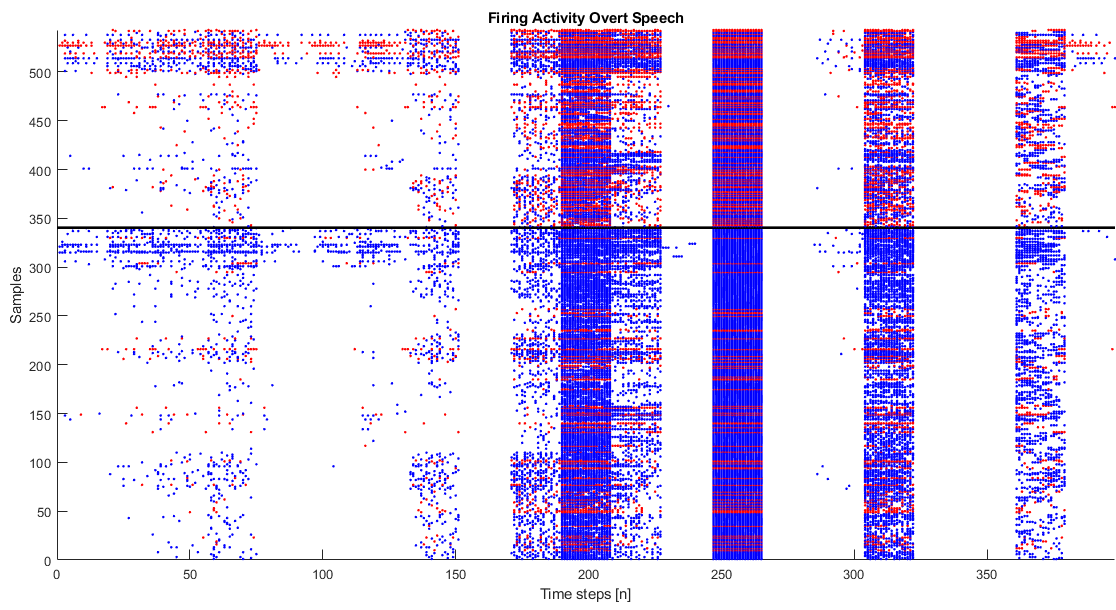
\includegraphics[width=\linewidth]{Figures/FA_SSN_Overt.png}
	\caption{Firing activity per sample class and misclassified samples highlighted after SSN testing for overt speech example.}
	\label{Fig: FA_SSN_Overt}
\end{figure}

\begin{figure}[h!]
	\centering
	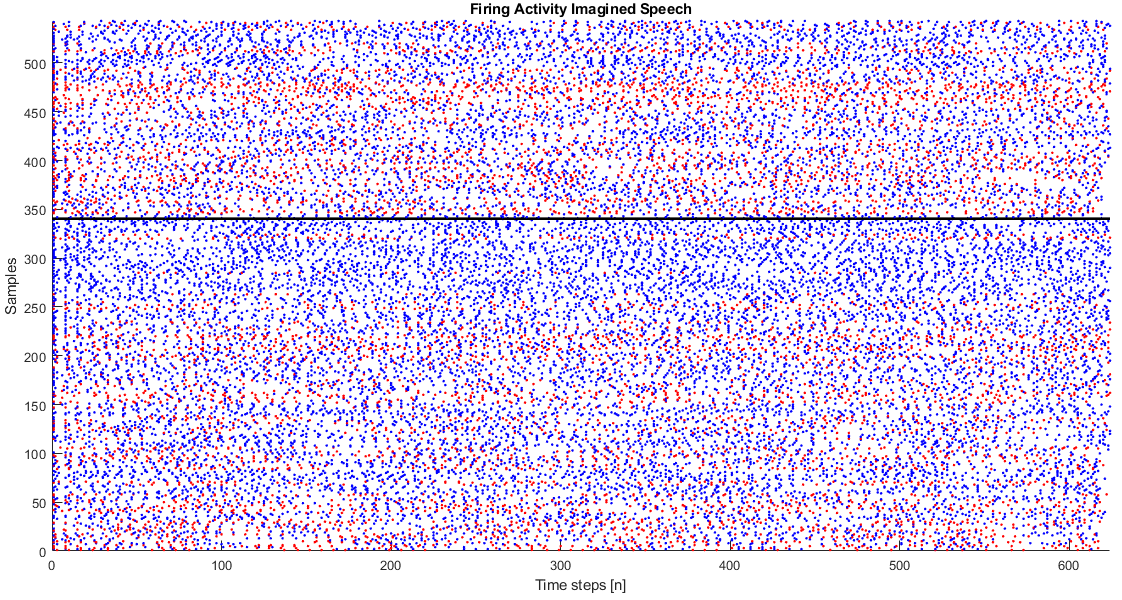
\includegraphics[width=\linewidth]{Figures/FA_SSN_Imagined.png}
	\caption{Firing activity per sample class and misclassified samples highlighted after SSN testing for imagined speech example.}
	\label{Fig: FA_SSN_Imagined}
\end{figure}

Besides, in the case of overt speech, the AFR associated to the class $-$Bilabial and $+$Bilabial were 0.1514 and 0.18.66, respectively; while for imagined speech, the AFR for class $-$Bilabial and $+$Bilabial were 0.0694 and 0.0725, respectively. Also, Figures \ref{Fig: Accuracies_SSN_Overt} and \ref{Fig: Accuracies_SSN_Imagined} show in different plots, for overt and imagined speech classification respectively, training and test accuracies (percentages) across the experiments by using $SSN_{L}$ and $SSN_{I}$ classifiers.\\

\begin{table}[h!]
	\centering
	\caption{Error percentages from the best results using SSN for overt speech.}
	\scalebox{0.8}{
	\begin{tabular}{|*{7}{c|}}
		\cline{2-7}
		\multicolumn{1}{c|}{\multirow{1}{*}{}} & \multicolumn{4}{c|}{\textbf{Vector-based}} & \multicolumn{2}{c|}{\multirow{2}{*}{\textbf{Spatio-tempora}l}} \\\cline{2-5}
		\multicolumn{1}{c|}{\multirow{1}{*}{}} & \multicolumn{2}{c|}{\textbf{3 features}} & \multicolumn{2}{c|}{\textbf{21 features}} & \multicolumn{2}{c|}{} \\\hline
		\textbf{Subjects} & $-$\textbf{Bilabial} & \boldmath$+$\textbf{Bilabial} & \boldmath$-$\textbf{Bilabial} & \boldmath$+$\textbf{Bilabial} & \boldmath$-$\textbf{Bilabial} & \boldmath$+$\textbf{Bilabial} \\\hline
		\boldmath$S_{1}$ & 12.94 & 46.31 & 2.36 & 69.95 & 10.88 & 65.03 \\\hline
		\boldmath$S_{2}$ & 14.12 & 44.34 & 2.36 & 69.46 & 9.71 & 56.65 \\\hline
		\boldmath$S_{3}$ & 7.65 & 55.67 & 2.65 & 73.89 & 8.82 & 57.64 \\\hline
		\boldmath$S_{4}$ & 6.76 & 57.64 & 2.36 & 70.44 & 8.53 & 57.14 \\\hline
		\boldmath$S_{5}$ & 9.12 & 62.56 & 2.06 & 69.95 & 11.47 & 49.75 \\\hline
		\textbf{Avg.}   & \textbf{10.12}\boldmath$\pm$\textbf{3.25} & \textbf{53.30}\boldmath$\pm$\textbf{7.74} & \textbf{2.36}\boldmath$\pm$\textbf{0.21} & \textbf{70.74}\boldmath$\pm$\textbf{1.8} & \textbf{9.88}\boldmath$\pm$\textbf{1.28} & \textbf{57.24}\boldmath$\pm$\textbf{5.41} \\\hline
	\end{tabular}%
	}
	\label{Table: Errors_SSN_Overt}%
\end{table}%

\begin{table}[h!]
\centering
\caption{Error percentages from the best results using SSN for imagined speech.}
\scalebox{0.8}{
\begin{tabular}{|*{7}{c|}}
	\cline{2-7}
	\multicolumn{1}{c|}{\multirow{1}{*}{}} & \multicolumn{4}{c|}{\textbf{Vector-based}} & \multicolumn{2}{c|}{\multirow{2}{*}{\textbf{Spatio-tempora}l}} \\\cline{2-5}
	\multicolumn{1}{c|}{\multirow{1}{*}{}} & \multicolumn{2}{c|}{\textbf{3 features}} & \multicolumn{2}{c|}{\textbf{21 features}} & \multicolumn{2}{c|}{} \\\hline
	\textbf{Subjects} & $-$\textbf{Bilabial} & \boldmath$+$\textbf{Bilabial} & \boldmath$-$\textbf{Bilabial} & \boldmath$+$\textbf{Bilabial} & \boldmath$-$\textbf{Bilabial} & \boldmath$+$\textbf{Bilabial} \\\hline
	\boldmath$S_{1}$ & 16.47 & 42.37 & 17.40 & 50.74 & 16.47 & 48.28 \\\hline
	\boldmath$S_{2}$ & 15.00 & 43.84 & 18.29 & 49.75 & 20.88 & 41.38 \\\hline
	\boldmath$S_{3}$ & 15.59 & 41.38 & 20.06 & 44.83 & 25.59 & 34.48 \\\hline
	\boldmath$S_{4}$ & 15.88 & 41.38 & 16.81 & 50.25 & 21.18 & 38.42 \\\hline
	\boldmath$S_{5}$ & 13.82 & 47.78 & 10.91 & 59.61 & 23.24 & 35.47 \\\hline
	\textbf{Avg.}   & \textbf{15.35}\boldmath$\pm$\textbf{1.01} & \textbf{43.35}\boldmath$\pm$\textbf{2.68} & \textbf{16.69}\boldmath$\pm$\textbf{3.46} & \textbf{51.03}\boldmath$\pm$\textbf{5.35} & \textbf{21.47}\boldmath$\pm$\textbf{3.37} & \textbf{39.61}\boldmath$\pm$\textbf{5.55} \\\hline
\end{tabular}%
}
\label{Table: Errors_SSN_Imagined}%
\end{table}%

\begin{figure}[h!]
\centering
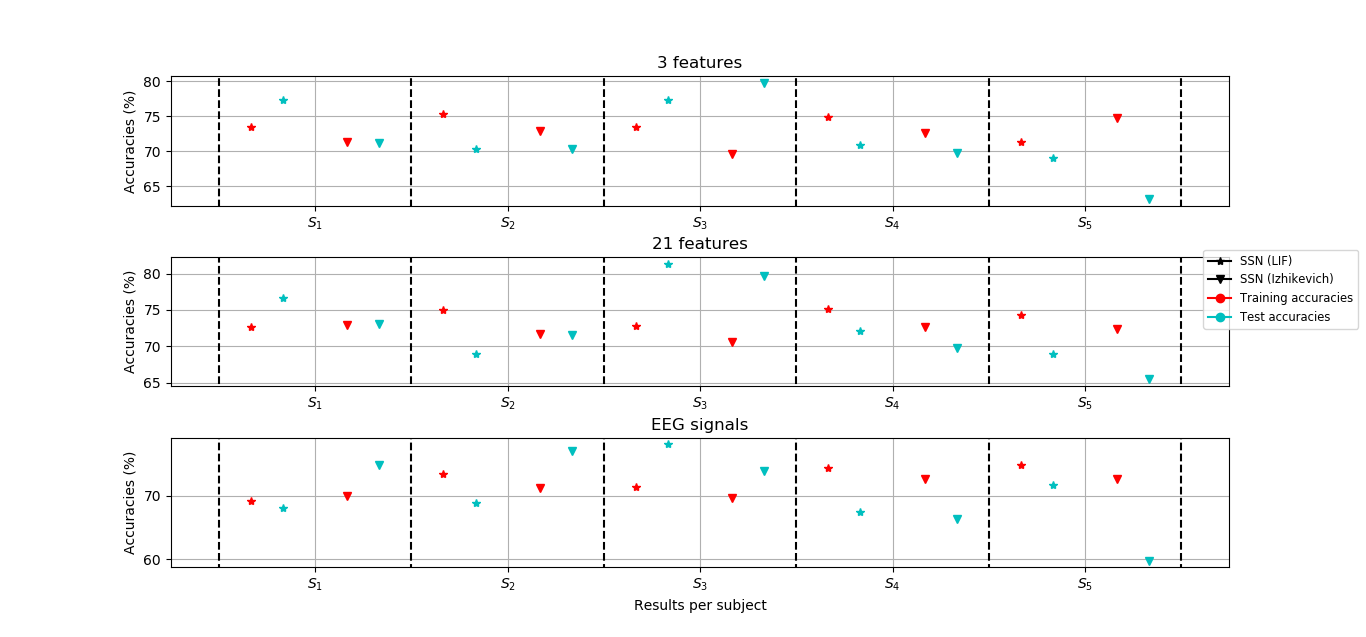
\includegraphics[width=\linewidth]{Figures/Accuracies_SSN_Overt.png}
\caption{Accuracies of the best configurations per case for overt speech samples.}
\label{Fig: Accuracies_SSN_Overt}
\end{figure}

In general, $SSN_{L}$ accuracies outperformed those obtained with $SSN_{I}$ for training and test data. Hence, the training accuracies were higher than those from test data in almost all cases. However, it happened the opposite in both Figures when $S_{3}$ data (and other subject's data in some particular cases) were held out.\\

These results mean that the classifiers could generalize better both mental activities with the rest data than with $S_{3}$ data, even though the training accuracies were lower than when other subject's data different from $S_{3}$ were held out.\\

\begin{figure}[h!]
	\centering
	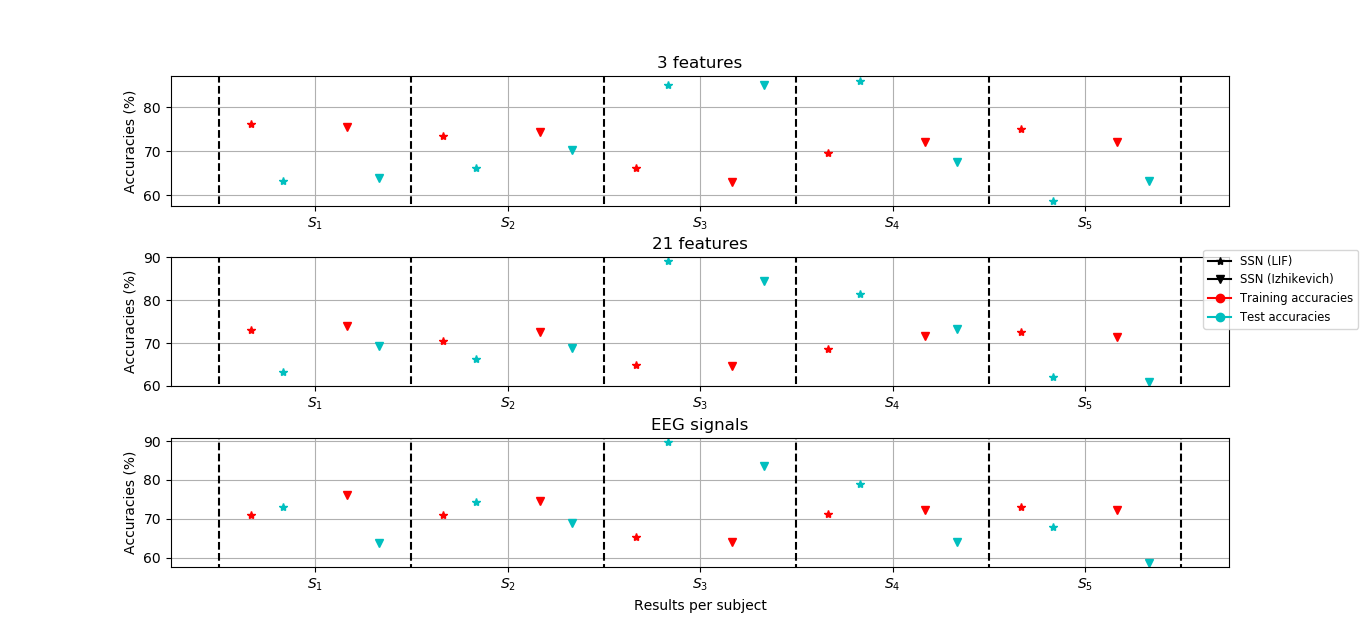
\includegraphics[width=\linewidth]{Figures/Accuracies_SSN_Imagined.png}
	\caption{Accuracies of the best configurations per case for imagined speech samples.}
	\label{Fig: Accuracies_SSN_Imagined}
\end{figure}

\begin{table}[h!]
\centering
\caption{Best scores obtained with $SSN_{L}$ for overt speech samples.}
\begin{tabular}{|*{8}{c|}}
	\cline{2-8}
	\multicolumn{1}{c|}{\multirow{1}{*}} & \textbf{Subject} & \boldmath$S_{1}$ & \boldmath$S_{2}$ & \boldmath$S_{3}$ & \boldmath$S_{4}$ & \boldmath$S_{5}$ & \textbf{Avg.} \\\hline
	\multirow{4}{*}{\begin{sideways}\textbf{Training}\end{sideways}} & \textbf{Accuracy} & 73.42 & 75.27 & 73.49 & 74.84 & 71.27 & \textbf{73.66}\boldmath$\pm$\textbf{1.56} \\\cline{2-8}
	& \textbf{Recall} & 76.06 & 77.02 & 73.42 & 73.48 & 70.94 & \textbf{74.18}\boldmath$\pm$\textbf{2.41} \\\cline{2-8}
	& \textbf{Precision} & 83.47 & 85.52 & 89.92 & 93.33 & 93.13 & \textbf{89.07}\boldmath$\pm$\textbf{4.45} \\\cline{2-8}
	& \textbf{F1} & 79.60 & 81.05 & 80.84 & 82.23 & 80.53 & \textbf{80.85}\boldmath$\pm$\textbf{0.95} \\\hline
	\multirow{4}{*}{\begin{sideways}\textbf{Test}\end{sideways}} & \textbf{Accuracy} & 77.30 & 70.27 & 77.34 & 70.93 & 68.97 & \textbf{72.96}\boldmath$\pm$\textbf{4.04} \\\cline{2-8}
	& \textbf{Recall} & 75.57 & 73.33 & 73.87 & 70.83 & 70.37 & \textbf{72.8}\boldmath$\pm$\textbf{2.17} \\\cline{2-8}
	& \textbf{Precision} & 95.19 & 88.00 & 100.00 & 92.73 & 77.55 & \textbf{90.69}\boldmath$\pm$\textbf{8.53} \\\cline{2-8}
	& \textbf{F1} & 84.26 & 80.00 & 84.97 & 80.31 & 73.79 & \textbf{80.67}\boldmath$\pm$\textbf{4.45} \\\hline
\end{tabular}%
\label{Table: Overt_Scores}%
\end{table}%

\begin{table}[h!]
\centering
\caption{Best scores obtained with $SSN_{L}$ for imagined speech samples.}
\begin{tabular}{|*{8}{c|}}
	\cline{2-8}
	\multicolumn{1}{c|}{\multirow{1}{*}} & \textbf{Subject} & \boldmath$S_{1}$ & \boldmath$S_{2}$ & \boldmath$S_{3}$ & \boldmath$S_{4}$ & \boldmath$S_{5}$ & \textbf{Avg.} \\\hline
	\multirow{4}{*}{\begin{sideways}\textbf{Training}\end{sideways}} & \textbf{Accuracy} & 71.05 & 71.00 & 65.30 & 71.12 & 73.03 & \textbf{70.3}\boldmath$\pm$\textbf{2.92} \\\cline{2-8}
	& \textbf{Recall} & 76.25 & 76.74 & 73.95 & 77.22 & 80.00 & \textbf{76.83}\boldmath$\pm$\textbf{2.17} \\\cline{2-8}
	& \textbf{Precision} & 77.54 & 76.21 & 68.22 & 76.14 & 76.98 & \textbf{75.02}\boldmath$\pm$\textbf{3.84} \\\cline{2-8}
	& \textbf{F1} & 76.89 & 76.47 & 70.97 & 76.68 & 78.46 & \textbf{75.89}\boldmath$\pm$\textbf{2.86} \\\hline
	\multirow{4}{*}{\begin{sideways}\textbf{Test}\end{sideways}} & \textbf{Accuracy} & 73.01 & 74.32 & 89.84 & 79.07 & 67.82 & \textbf{76.81}\boldmath$\pm$\textbf{8.31} \\\cline{2-8}
	& \textbf{Recall} & 71.13 & 73.85 & 90.59 & 78.46 & 69.81 & \textbf{76.77}\boldmath$\pm$\textbf{8.41} \\\cline{2-8}
	& \textbf{Precision} & 97.12 & 96.00 & 93.90 & 92.73 & 75.51 & \textbf{91.05}\boldmath$\pm$\textbf{8.86} \\\cline{2-8}
	& \textbf{F1} & 82.11 & 83.48 & 92.22 & 85.00 & 72.55 & \textbf{83.07}\boldmath$\pm$\textbf{7.06} \\\hline
\end{tabular}%
\label{Table: Imagined_Scores}%
\end{table}%

Moreover, the plots from Figure \ref{Fig: Accuracies_SSN_Overt} corresponding to Vector-based experiments presented similar results. For this reason and due to less required computations, the scores from 3 feature vector experiments with $SSN_{L}$ were considered in this work as the best obtained for overt speech samples. On the other hand, the scores from Spatio-temporal experiments with $SSN_{L}$ were regarded as the best obtained for imagined speech samples.\\

Tables \ref{Table: Overt_Scores} and \ref{Table: Imagined_Scores} show in detail these best scores obtained from overt and imagined speech experiments, respectively. These scores consisted of the accuracy, recall, precision, and F1 per subject's data held out from the rest.\\

Besides, the averages$\pm$standard deviations are shown across the experiments per score, which show, for both mental activities, that the variations in all training scores remained low, while test scores variations were high (mainly because of $S_{3}$ data results). These low variations in the training scores show that, for both mental activities, the $SSN_{L}$ learning capacity is similar when different training samples are used.\\

Finally, Figures \ref{Fig: CM_Overt} and  \ref{Fig: CM_Imagined} show the confusion matrices from which the best scores of imagined and overt speech, respectively, were extracted. In the case of overt speech (Figure \ref{Fig: CM_Overt}), almost all the samples (correctly or incorrectly) were classified as  $-$Bilabial(the range values are from 0 to 1). Although the least unbalanced binary configuration was used, the amount of $-$Bilabial samples (340 against 203) aided the scores to be higher than 70\%.\\

On the other hand, in the case of imagined speech training samples (first column of Figure \ref{FIg: CM_Imagined}), the recognition rate of both classes was balanced and slightly high on average (76\% for $-$Bilabial and 60\% for  $+$Bilabial). While, the same situation as for overt speech happened with test samples, except when $S_{3}$ data was used, which provided high recognition rates for both classes (94\% for $-$Bilabial and 83\% for  $+$Bilabial).\\

To sum up, the classification rates for both mental activities were above 70\%, although the unbalance between class samples aided to achieve these results. Besides, imagined speech classification rates outperformed those from overt speech, possibly due to the amount of temporal information used in the SSN (625 sample points against 57 features). These results agreed with those from \cite{salinas2017bag}, in which the best scores for imagined speech were obtained with EEG raw data. Hence, these results show the importance of designing new acquisition experiments, as well as the necessity of collecting new balanced samples. These aspects are summarized in the next chapter.

\begin{figure}[h!]
	\centering
	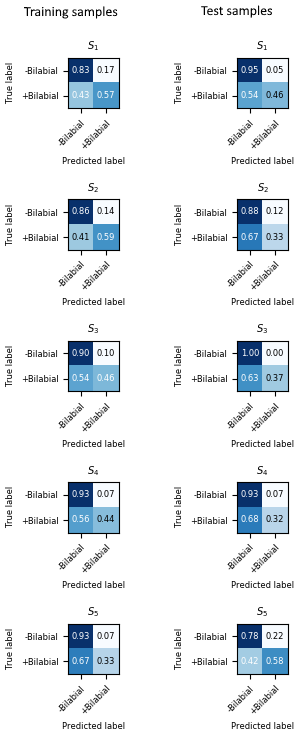
\includegraphics[scale=1.2]{Figures/CM_Overt.png}
	\caption{Confusion matrices from best overt speech scores.}
	\label{Fig: CM_Overt}
\end{figure}

\begin{figure}[h!]
\centering
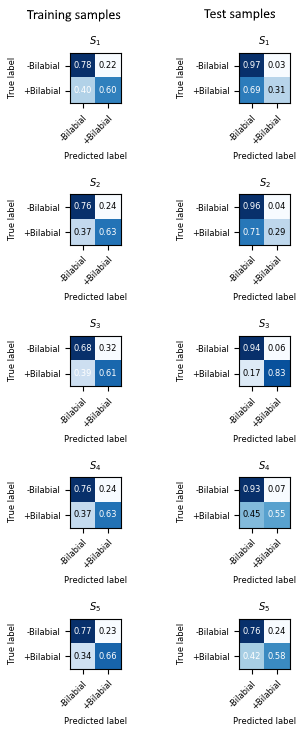
\includegraphics[scale=1.2]{Figures/CM_Imagined.png}
\caption{Confusion matrices from best imagined speech scores.}
\label{Fig: CM_Imagined}
\end{figure}